\documentclass{standalone}
\usepackage{graphicx}	
\usepackage{amssymb, amsmath}
\usepackage{color}

\usepackage{tikz}
\usetikzlibrary{intersections, backgrounds}
\usepackage{pgfmath}

\definecolor{light}{RGB}{220, 188, 188}
\definecolor{mid}{RGB}{185, 124, 124}
\definecolor{dark}{RGB}{143, 39, 39}
\definecolor{highlight}{RGB}{180, 31, 180}
\definecolor{gray10}{gray}{0.1}
\definecolor{gray20}{gray}{0.2}
\definecolor{gray30}{gray}{0.3}
\definecolor{gray40}{gray}{0.4}
\definecolor{gray60}{gray}{0.6}
\definecolor{gray70}{gray}{0.7}
\definecolor{gray80}{gray}{0.8}
\definecolor{gray90}{gray}{0.9}
\definecolor{gray95}{gray}{0.95}

\begin{document}

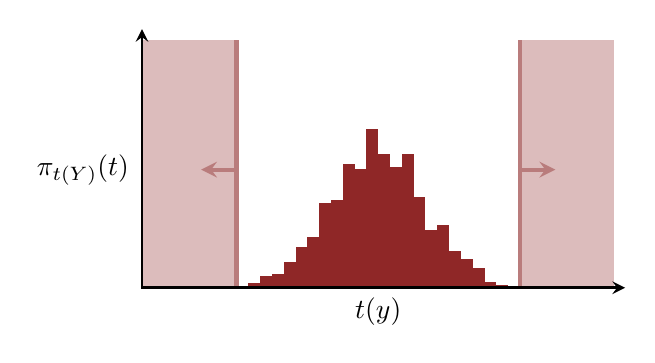
\begin{tikzpicture}[scale=0.3, thick]

  \foreach[count=\n] \y in {0.000, 0.000, 0.000, 0.000, 0.000, 0.000, 0.000, 0.002, 
                0.002, 0.006, 0.016, 0.020, 0.036, 0.058, 0.072, 0.120, 
                0.124, 0.174, 0.168, 0.224, 0.188, 0.170, 0.188, 0.128, 
                0.082, 0.088, 0.052, 0.040, 0.028, 0.008, 0.004, 0.002, 
                0.000, 0.000, 0.000, 0.000, 0.000, 0.000, 0.000, 0.000} {
    \fill[dark] ({(\n - 1) / 2 - 10}, 0) rectangle ({(\n) / 2 - 10}, {30 * \y});
  }

  \node[] at (-12.5, 5) { $\pi_{t(Y)} (t)$ };

  \fill[color=light] (-10, 0) rectangle (-6, 10.5);
  \draw[-, color=mid, line width=1.5] (-6, 0) -- (-6, 10.5);
  \draw[->, >=stealth, line width=1.5, color=mid] (-6, 5) -- +(-1.5, 0);

  \fill[color=light] (10, 0) rectangle (6, 10.5);
  \draw[-, color=mid, line width=1.5] (6, 0) -- (6, 10.5);
  \draw[->, >=stealth, line width=1.5, color=mid] (6, 5) -- +(1.5, 0);

  \draw [->, >=stealth, line width=1] (-10.05, 0) -- +(20.5, 0);
  \draw [->, >=stealth, line width=1] (-10, -0.05) -- +(0, 11);
  \node[] at (0, -1) { $t(y)$ };
  
  
  
\end{tikzpicture}

\end{document}  